\documentclass[a4paper,14pt]{extarticle}

% Путь до папки с общими шаблонами
\newcommand{\pathToCommonFolder}{/home/denilai/Documents/repos/latex/Common}
% Название работы в титуле
\newcommand{\workname}{Отчет по практическим работам 5-8}
% Название дисциплины в титуле
\newcommand{\discipline}{Технологические основы Инетернета вещей}
% Название кафедры в титуле
\newcommand{\kafedra}{Кафедра Математического обеспечения и стандартизации информационных технологий}
% Тема работы в титуле
\newcommand{\theme}{Знакомство с оборудованием}
% Должность преподавателя в титуле
\newcommand{\rang}{ассистент}

% ФИО студента в титуле
\newcommand{\studentfio}{К.~Ю.~Денисов}%\\Д.~Н.~Федосеев\\А.~М.~Сосунов}\\%К.~Ю.~Денисов\\%И.~А.~Кремнев
% ФИО преподавателя в титуле
\newcommand{\teacherfio}{Ю.~А.~Воронцов}


\usepackage{tabularx}


\usepackage{booktabs}
\newcolumntype{b}{X}
\newcolumntype{s}{>{\hsize=.5\hsize}X}
\newcommand{\heading}[1]{\multicolumn{1}{c}{#1}}

% установка размера шрифта для всего документа
%\fontsize{20pt}{18pt}\selectfont
\usepackage{extsizes} % Возможность сделать 14-й шрифт

% Вставка заготовки преамбулы
% Этот шаблон документа разработан в 2014 году
% Данилом Фёдоровых (danil@fedorovykh.ru) 
% для использования в курсе 
% <<Документы и презентации в \LaTeX>>, записанном НИУ ВШЭ
% для Coursera.org: http://coursera.org/course/latex .
% Исходная версия шаблона --- 
% https://www.writelatex.com/coursera/latex/5.3

% В этом документе преамбула

% Для корректного использования русских символов в формулах
% пакеты hyperref и настройки, связанные с ним, стоит загуржать
% перед загрузкой пакета mathtext



% поддержка русских букв
% кодировка шрифта
%\usepackage[T2A]{fontenc} 
\usepackage{pscyr}

% использование ненумеровонного абзаца с добавлением его в содержаниеl

\newcommand{\anonsection}[1]{\section*{#1}\addcontentsline{toc}{section}{#1}}
\newcommand{\sectionunderl}[1]{\section*{\underline{#1}}}


% настройка окружения enumerate
\usepackage{enumitem}
\setlist{noitemsep}
\setlist[enumerate]{labelsep=*, leftmargin=1.5pc}

\usepackage{hyperref}

% сначала ставить \usepackage{extsizes} % Возможность сделать 14-й шрифт
% для корректной установки полей вставлять преамбулу следует в последнюю очередь (но перед дерективой замены \rmdefault)
\usepackage[top=20mm,bottom=25mm,left=35mm,right=20mm]{geometry} % Простой способ задавать поля

\hypersetup{				% Гиперссылки
	unicode=true,           % русские буквы в раздела PDF
	pdftitle={Заголовок},   % Заголовок
	pdfauthor={Автор},      % Автор
	pdfsubject={Тема},      % Тема
	pdfcreator={Создатель}, % Создатель
	pdfproducer={Производитель}, % Производитель
	pdfkeywords={keyword1} {key2} {key3}, % Ключевые слова
	colorlinks=true,       	% false: ссылки в рамках; true: цветные ссылки
	linkcolor=red,          % внутренние ссылки
	citecolor=black,        % на библиографию
	filecolor=magenta,      % на файлы
	urlcolor=blue           % на URL
}

%%% Работа с русским языком
\usepackage{cmap}					% поиск в PDF
\usepackage{mathtext} 				% русские буквы в формулах
\usepackage[T2A]{fontenc}			% кодировка
\usepackage[utf8]{inputenc}			% кодировка исходного текста
\usepackage[english,russian]{babel}	% локализация и переносы
\usepackage{indentfirst}
\frenchspacing

%для изменения названия списка иллюстраций
\usepackage{tocloft}


\renewcommand{\epsilon}{\ensuremath{\varepsilon}}
\renewcommand{\phi}{\ensuremath{\varphi}}
\renewcommand{\kappa}{\ensuremath{\varkappa}}
\renewcommand{\le}{\ensuremath{\leqslant}}
\renewcommand{\leq}{\ensuremath{\leqslant}}
\renewcommand{\ge}{\ensuremath{\geqslant}}
\renewcommand{\geq}{\ensuremath{\geqslant}}
\renewcommand{\emptyset}{\varnothing}

% Изменения параметров списка иллюстраций
\renewcommand{\cftfigfont}{Рисунок } % добавляем везде "Рисунок" перед номером
\addto\captionsrussian{\renewcommand\listfigurename{Список иллюстративного материала}}

\newcommand{\tm}{\texttrademark\ }
\newcommand{\reg}{\textregistered\ }


%%% Дополнительная работа с математикой
\usepackage{amsmath,amsfonts,amssymb,amsthm,mathtools} % AMS
\usepackage{icomma} % "Умная" запятая: $0,2$ --- число, $0, 2$ --- перечисление

%% Номера формул
%\mathtoolsset{showonlyrefs=true} % Показывать номера только у тех формул, на которые есть \eqref{} в тексте.
%\usepackage{leqno} % Нумереация формул слева

%% Свои команды
\DeclareMathOperator{\sgn}{\mathop{sgn}}

%% Перенос знаков в формулах (по Львовскому)
\newcommand*{\hm}[1]{#1\nobreak\discretionary{}
{\hbox{$\mathsurround=0pt #1$}}{}}


% отступ для первого абзаца главы или параграфа
%\usepackage{indentfirst}

%%% Работа с картинками
\usepackage{graphicx}  % Для вставки рисунков
\graphicspath{{images/}{screnshots/}}  % папки с картинками
\DeclareGraphicsExtensions{.pdf,.png,.jpg}
\setlength\fboxsep{3pt} % Отступ рамки \fbox{} от рисунка
\setlength\fboxrule{1pt} % Толщина линий рамки \fbox{}
\usepackage{wrapfig} % Обтекание рисунков текстом

%%% Работа с таблицами
\usepackage{array,tabularx,tabulary,booktabs} % Дополнительная работа с таблицами
\usepackage{longtable}  % Длинные таблицы
\usepackage{multirow} % Слияние строк в таблице

%%% Теоремы
\theoremstyle{plain} % Это стиль по умолчанию, его можно не переопределять.
\newtheorem{theorem}{Теорема}[section]
\newtheorem{proposition}[theorem]{Утверждение}

\theoremstyle{plain} % Это стиль по умолчанию, его можно не переопределять.
\newtheorem{work}{Практическая работа}[part]


 
 
\theoremstyle{definition} % "Определение"
\newtheorem{corollary}{Следствие}[theorem]
\newtheorem{problem}{Задача}[section]
 
\theoremstyle{remark} % "Примечание"
\newtheorem*{nonum}{Решение}



%%% Программирование
\usepackage{etoolbox} % логические операторы

%%% Страница

%	\usepackage{fancyhdr} % Колонтитулы
% 	\pagestyle{fancy}
%   \renewcommand{\headrulewidth}{0pt}  % Толщина линейки, отчеркивающей верхний колонтитул
% 	\lfoot{Нижний левый}
% 	\rfoot{Нижний правый}
% 	\rhead{Верхний правый}
% 	\chead{Верхний в центре}
% 	\lhead{Верхний левый}
%	\cfoot{Нижний в центре} % По умолчанию здесь номер страницы

\usepackage{setspace} % Интерлиньяж
\onehalfspacing % Интерлиньяж 1.5
%\doublespacing % Интерлиньяж 2
%\singlespacing % Интерлиньяж 1

\usepackage{lastpage} % Узнать, сколько всего страниц в документе.

\usepackage{soul} % Модификаторы начертания


\usepackage[usenames,dvipsnames,svgnames,table,rgb]{xcolor}


\usepackage{csquotes} % Еще инструменты для ссылок

%\usepackage[style=authoryear,maxcitenames=2,backend=biber,sorting=nty]{biblatex}

\usepackage{multicol} % Несколько колонок

\usepackage{tikz} % Работа с графикой
\usepackage{pgfplots}
\usepackage{pgfplotstable}

% модуль для вставки рыбы
\usepackage{blindtext}

\usepackage{listings}
\usepackage{color}


% для поворота отдельной страницы. Использовать окружение \landscape
\usepackage{pdflscape} 
\usepackage{rotating} 


\definecolor{mygreen}{rgb}{0,0.6,0}
\definecolor{mygray}{rgb}{0.5,0.5,0.5}
\definecolor{mymauve}{rgb}{0.58,0,0.82}


% пример импорта файла
%\lstinputlisting{/home/denilai/repomy/conf/distributions}

\lstset{
	language=Python,
	basicstyle=\footnotesize,        % the size of the fonts that are used for the code
	numbers=left,                    % where to put the line-numbers; possible values are (none, left, right)
	numbersep=5pt,                   % how far the line-numbers are from the code
	numberstyle=\tiny\color{mygray}, % the style that is used for the line-numbers
	stepnumber=2,                    % the step between two line-numbers. If it's 1, each line will be numbered
	% Tab - 2 пробела
	tabsize=2,    
	% Автоматический перенос строк
	breaklines=true,
	frame=single,
	breakatwhitespace=true,
	title=\lstname 
}



\author{Кирилл Денисов}
\title{Лабораторная работа №1}
\date{\today}

\renewcommand{\withouttheme}{1}

%если нужна тема работы в отчете, то указать в скобках что-либо, иначе оаставить пустым
%\renewcommand{\withouttheme}{}
%если нужна дата представления отчета, то указать в скобках что-либо
%\renewcommand{\withoutsubmissiondate}{1}

% установка полуторного интервала
% \usepackage{setspace}  
% \onehalfspacing

% использовать Times New Roman
\renewcommand{\rmdefault}{ftm}


\begin{document}
	\thispagestyle{empty}
	% Вставка первого титульного листа
	% Есть две версии титульного листа - одиночный (titul) и групповой (titulAll)
	%\newcommand{\withouttheme}{} добавить эту переменную для определения, нужна ли тема
%     {} - нужна
%    {1} - не нужна

%\newcommand{\withoutsubmissiondate}{} добавить эту переменную для определения, нужен ли срок предоставления отчета
%     {} - нужен
%    {1} - не нужен

\renewcommand{\studentfio}{К.~Ю.~Денисов\\
			%	& & \hfill И.~А.~Кремнев \\
				& & \hfill А.~М.~Сосунов\\
				& & \hfill Д.~Н.~Федосеев}

\begin{center}
	\begin{figure}[h!]
		\begin{center}
			%\vspace{10ex}
			
\includegraphics[width=0.17\linewidth]{\pathToCommonFolder/gerb}
			%\caption{}\label{pic:first}
			%	\vspace{5ex}
		\end{center}	
	\end{figure}
	\small	МИНОБРНАУКИ РОССИИ \\
	Федеральное государственное бюджетное образовательное учреждение\\
	высшего образования\\
	\normalsize					
	\textbf{«МИРЭА – Российский технологический университет»\\
		РТУ МИРЭА}\\
	\noindent\rule{1\linewidth}{1pt}\\
	Институт информационных технологий\\ %\vspace{2ex}
	\kafedra\\
	\vspace{3ex}
	\large \textbf{\workname}  \\
	%\vspace{1ex}
	по дисциплине\\ «\discipline» \\
	\vspace{3ex}
	\if \withouttheme
	\textbf{Тема работы:}\\ <<\theme>>
	\fi
	\vspace{6ex}
	\small
	\begin{table}[h!]
		\begin{tabular}{lp{0.6\linewidth}l}
			\textbf{Выполнили:} & студенты группы ИВБО-02-19 & \\ 
			& & \hfill \studentfio \\%Д.~Н.~Федосеев\\%А.~М.~Сосунов\\%К.~Ю.~Денисов\\%И.~А.~Кремнев
			\textbf{Принял:} & \rang & \\
			& & \hfill \teacherfio\\
		\end{tabular}
	\end{table}

	\normalsize
	
	\vfill
	Москва 2021
	
\end{center}
	\newpage
	\tableofcontents
	\newpage
	%\listoftables

\normalsize

\section{Практическая работа №5.\\Измерительные и исполнительные устройства в Интернете вещей}

\subsection {Измерительные \\и исполнительные устройства стенда}
Работа на практических занятиях проводится с использованием стенда (чемодана\textbf{ WBdemo-kit v.2}), содержащего типовой набор оборудования в <<умном доме>>.

Стенд состоит из компонентов, расположение которых можно увидеть на Рис. \ref{fig:wb-demo-kit1}-\ref{fig:wb-demo-kit2}. В таблице \ref{tab:device-list} приводится их полный список.
 
% TODO: \usepackage{graphicx} required
\begin{figure}[htpb]
	\centering
	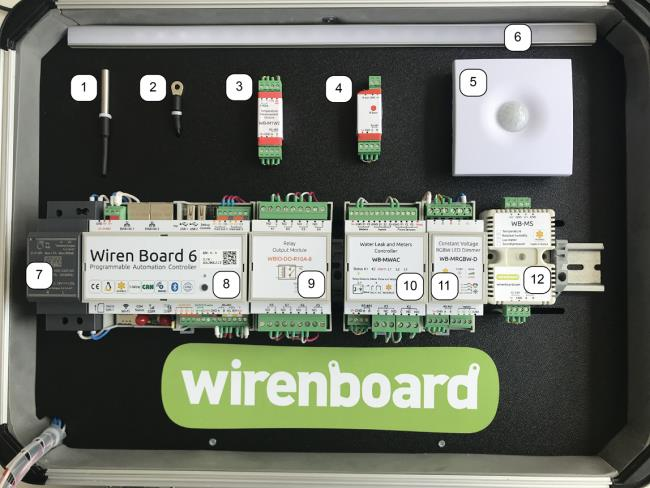
\includegraphics[width=0.6\linewidth]{images/wb-demo-kit1}
	\caption{Компоненты, расположенные на верхней крышке WB-demo-kit}
	\label{fig:wb-demo-kit1}
\end{figure}
 
 % TODO: \usepackage{graphicx} required
 \begin{figure}[htpb]
 	\centering
 	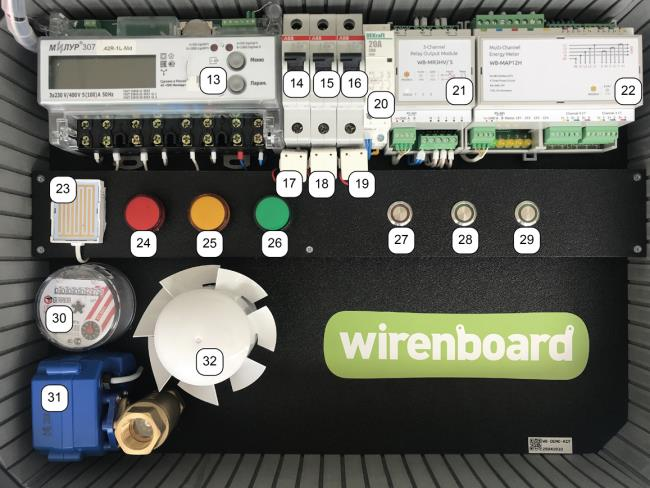
\includegraphics[width=0.6\linewidth]{images/wb-demo-kit2}
 	\caption{Компоненты, расположенные на нижней крышке WB-demo-kit}
 	\label{fig:wb-demo-kit2}
 \end{figure}

\begin{center}
	\begin{table}[htbp]
	%\small
	\begin{tabular}{|r|p{0.8\linewidth}|}
		\hline
		\multicolumn{1}{|c|}{\textbf{Номер}} & \multicolumn{1}{c|}{\textbf{Название}} \\ \hline\hline
		1 & Датчик температуры 1-wire DS18B20 \\ \hline
		2 & Датчик температуры 1-wire DS18B20 \\ \hline
		4 & Устройство ИК-управления WB-MIR \\ \hline
		5 & Настенный комбинированный датчик WB-MSW v.3 \\ \hline
		10 & Модуль обнаружения протечек WB-MWAC \\ \hline
		11 & Диммер светодиодных лент на DIN-рейку WB-MRGBW-D \\ \hline
		12 & Комбинированный датчик WB-MS \\ \hline
		21 & Модуль реле 3-канальный WB-MR3 \\ \hline
		22 & Многоканальный измеритель WB-MAP12H \\ \hline
		23 & Датчик протечки \\ \hline
	\end{tabular}
    \caption{Список датчиков и исполнительных устройств демонстрационного набора WB-demo-kit}
	\label{tab:device-list}
\end{table}
\end{center}



	
\subsection*{Индивидуальный вариант №5}
В ходе выполнения данной практической работы были изучены датчики и исполнительные устройства \textbf{Wb-demo-kit v.2}:

\begin{enumerate}
	\item Освещенность в составе датчика WB-MSW v.3 (5)
	\item Влажность в составе датчика WB-MS v.2 (12)
	\item Преобразователь 1-Wire — Modbus RTU WB-M1W2 (3)
\end{enumerate}

Опишем устройства в отдельности
\subsubsection*{Освещенность в составе датчика WB-MSW v.3 (5)}

\begin{enumerate}
	\item \textbf{Название датчика/устройства:} датчик освещения в составе WB-MSW v.3
	
	\item \textbf{Тип измерения:} цифровой
	
	\item  \textbf{Измеряемые параметры и диапазон измерения:} Освещённость; 0,02~--~100 000 лк
	
	\item  \textbf{Точность:} $\pm10 \%$	
	\item  \textbf{Напряжение питания:} 9 В~--~28 В постоянного тока
	
	\item  \textbf{Уникальный идентификатор датчика в веб-интерфейсе:} \\wb-msw-v3\_21/Illuminance
	
	\item  \textbf{Использующийся протокол передачи данных:} Modbus RTU
	
	\item  \textbf{Интерфейс управления (шина):} RS-485
	
	\item  \textbf{Описание входов и выходов, схема подключения:} см. рис. \ref{fig:device-1}.
\end{enumerate}


\subsubsection*{Влажность в составе датчика WB-MS v.2 (12)}
\begin{enumerate}
	\item \textbf{Название датчика/устройства:} датчик влажности в составе WB-MS v.2
	
	\item \textbf{Тип измерения:} цифровой
	
	\item  \textbf{Измеряемые параметры и диапазон измерения:} влажность; 0~–~98~\%
	
	\item  \textbf{Точность:} $\pm3 \%$	
	\item  \textbf{Напряжение питания:} 9 В~--~28 В постоянного тока
	
	\item  \textbf{Уникальный идентификатор датчика в веб-интерфейсе:} \\wb-ms\_11/Humidity
	
	\item  \textbf{Использующийся протокол передачи данных:} Modbus RTU
	
	\item  \textbf{Интерфейс управления (шина):} RS-485
	
	\item  \textbf{Описание входов и выходов, схема подключения:} см. рис. \ref{fig:device-2}.
	
\end{enumerate}

\subsubsection*{Преобразователь 1-Wire~--~Modbus RTU WB-M1W2}
\begin{enumerate}
	\item \textbf{Название датчика/устройства:} компактный преобразователь2
	
	\item \textbf{Тип измерения:} цифровой
	
	\item  \textbf{Напряжение питания:} 9 В~--~28 В постоянного тока
	
	\item  \textbf{Уникальный идентификатор датчика в веб-интерфейсе:}\\ wb-m1w2\_14
	
	\item  \textbf{Использующийся протокол передачи данных:} Modbus RTU
	
	\item  \textbf{Интерфейс управления (шина):} RS-485
	
	\item  \textbf{Описание входов и выходов, схема подключения:} см. рис. \ref{fig:device-3}.
	
\end{enumerate}

	% TODO: \usepackage{graphicx} required
\begin{figure}[h!]
	\centering
	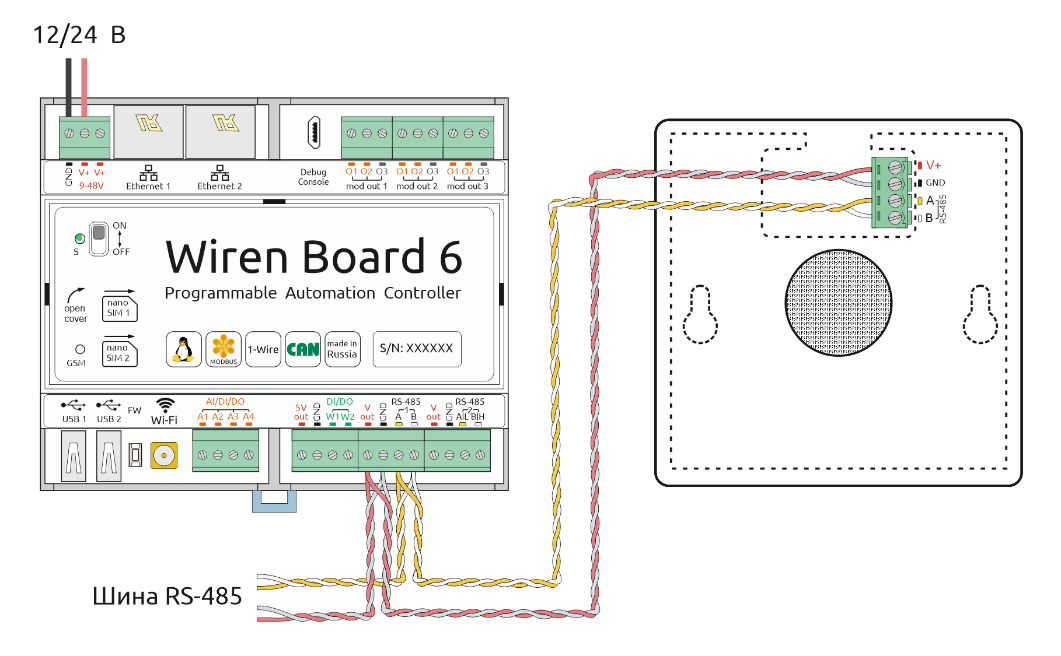
\includegraphics[width=0.5\linewidth]{images/device-1}
	\caption{Датчик освещенности}
	\label{fig:device-1}
\end{figure}

% TODO: \usepackage{graphicx} required
\begin{figure}[h!]
	\centering
	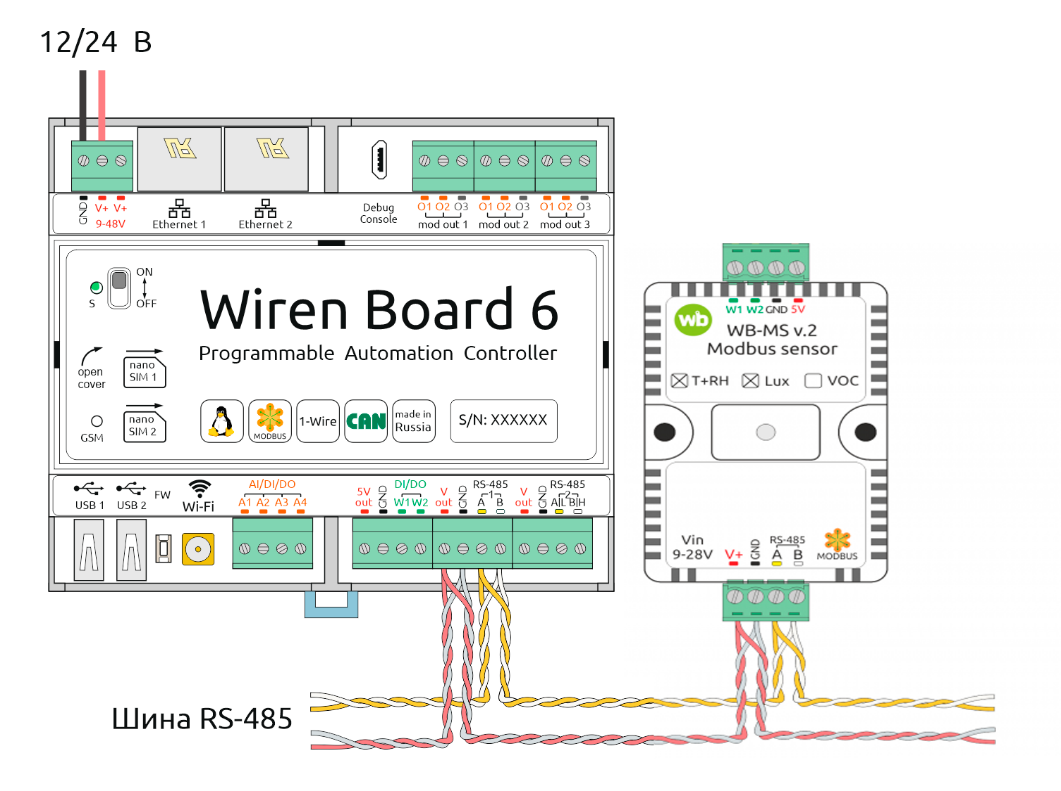
\includegraphics[width=0.5\linewidth]{images/device-2}
	\caption{Датчик влажности}
	\label{fig:device-2}
\end{figure}

% TODO: \usepackage{graphicx} required
\begin{figure}[h!]
	\centering
	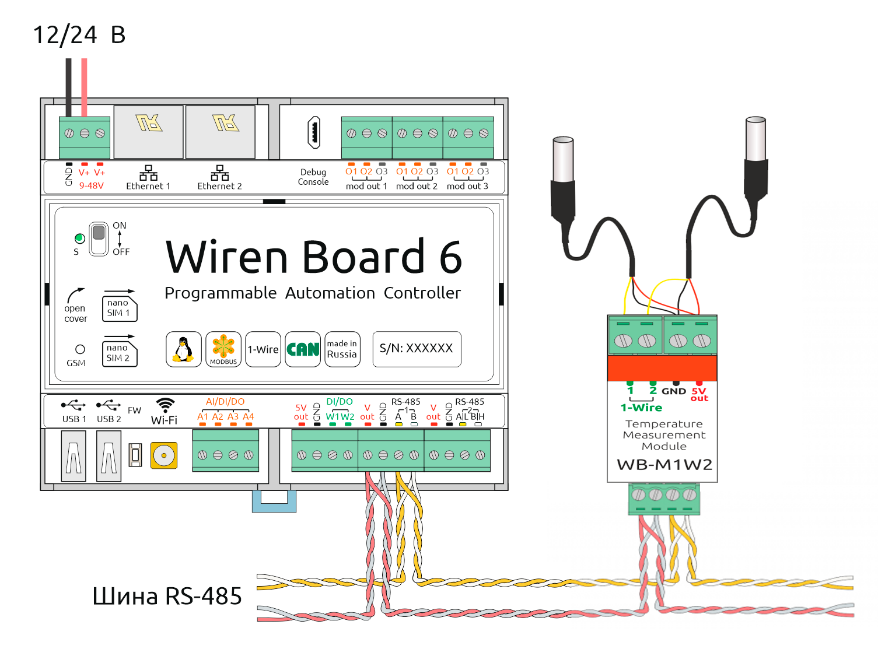
\includegraphics[width=0.5\linewidth]{images/device-3}
	\caption{Преобразователь 1--Wire~—~Modbus RTU}
	\label{fig:device-3}
\end{figure}

\newpage
\subsection{Протоколы работы с устройствами}


Опишем принцип работы, преимущества и недостатки, сферу применения следующих
четырех технологий:
\begin{enumerate}
	\item Modbus RTU;
	\item  1-Wire;
	\item  I${}^2$C (IIC, англ. Inter-Integrated Circuit);
	\item  CAN.
\end{enumerate}

\subsubsection*{Modbus RTU}

Modbus --- коммуникационный протокол, основан на архитектуре ведущий-ведомый (master-slave). Использует для передачи данных интерфейсы RS-485, RS-422, RS-232, а также Ethernet сети TCP/IP (протокол Modbus TCP).

Сообщение Modbus RTU состоит из адреса устройства SlaveID, кода функции, специальных данных в зависимости от кода функции и CRC контрольной суммы.

SlaveID – это адрес устройства, может принимать значение от 0 до 247, адреса с 248 до 255 зарезервированы.

\paragraph*{Достоинства стандарта}
Основные достоинства стандарта — открытость и массовость. Промышленностью сейчас (2014 г.) выпускается очень много типов и моделей датчиков, исполнительных устройств, модулей обработки и нормализации сигналов и др. Практически все промышленные системы контроля и управления имеют программные драйверы для работы с MODBUS-сетями.

\paragraph*{Недостатки стандарта}
Стандарт в своей основе был разработан в 1979 году с учётом потребностей и вычислительных возможностей того времени, и многие актуальные для современных промышленных сетей вопросы не были учтены. Необходимо отметить, что отсутствие перечисленных возможностей является следствием простоты протокола, которая облегчает его изучение и ускоряет внедрение.

\begin{itemize}
	\item Стандарт специфицирует метод передачи только двух типов данных. 
	\item Стандарт не регламентирует начальную инициализацию системы.
	\item Не предусмотрена передача сообщений по инициативе подчинённого устройства (прерываний). 
	\item Длина запроса ограничена, а данные могут быть запрошены только из последовательно расположенных регистров. 
	\item Не предусмотрен способ, с помощью которого подчинённое устройство могло бы обнаружить потерю связи с ведущим.
\end{itemize}



\subsubsection*{1-Wire}
1-Wire c (англ. --- <<один провод>>) --- двунаправленная шина связи для устройств с низкоскоростной передачей данных (обычно 15,4 Кбит/с, максимум 125 Кбит/с в режиме overdrive), в которой данные передаются по цепи питания (то есть всего используются два провода — один общий (GND), а второй для питания и данных; в некоторых случаях используют и отдельный провод питания). Разработана корпорацией Dallas Semiconductor.

Соответственно, топология такой сети --- общая шина. Сеть устройств 1-Wire со связанным основным устройством названа «MicroLan», это также торговая марка Dallas Semiconductor.

Обычно используется для того, чтобы связываться с недорогими простыми устройствами, такими, как, например, цифровые термометры и измерители параметров внешней среды.

\paragraph*{Достоинства}

\begin{itemize}
	\item Для связи с устройством требуется лишь два провода: на данные и заземление. Интегральная схема включает конденсатор ёмкостью 800 пФ для питания от линии данных (так называемое паразитное питание).
		\item Большое расстояние передачи. Расстояние достигает 300 м при соблюдении ряда условий:
		\begin{itemize}
			\item применение кабеля типа «витая пара»;
			\item использование специального драйвера сети (активная подтяжка с учётом тока в линии);
			\item использование топологии «общая шина» с единым стволом (не свободная топология);
		\end{itemize}
	
		\item Изменяемость конфигурации любой сети 1-Wire в процессе её работы.
\end{itemize}

\paragraph*{Недостатки}
\begin{itemize}
	\item Низкая скорость передачи данных;
	\item Проводной интерфейс. Хотя в конкретном случае это может быть и достоинством.
\end{itemize}


\subsection*{I${}^2$C }
I${}^2$C (IIC), (Inter-Integrated Circuit)  --- последовательная асимметричная шина для связи между интегральными схемами внутри электронных приборов. Использует две двунаправленные линии связи (SDA и SCL), применяется для соединения низкоскоростных периферийных компонентов с процессорами и микроконтроллерами (например, на материнских платах, во встраиваемых системах, в мобильных телефонах).

\paragraph{Принцип работы}
I${}^2$C использует две двунаправленные линии, подтянутые к напряжению питания и управляемые через открытый коллектор или открытый сток — последовательная линия данных (SDA, англ. Serial DAta) и последовательная линия тактирования (SCL, англ. Serial CLock). Стандартные напряжения +5 В или +3,3 В, однако допускаются и другие.

Классическая адресация включает 7-битное адресное пространство с 16 зарезервированными адресами. Это означает, что разработчикам доступно до 112 свободных адресов для подключения периферии на одну шину.

Основной режим работы — 100 кбит/с; 10 кбит/с в режиме работы с пониженной скоростью. Также немаловажно, что стандарт допускает приостановку тактирования для работы с медленными устройствами.

\paragraph*{Преимущества}
\begin{enumerate}
	\item необходим всего один микроконтроллер для управления набором устройств;
	\item используется всего два проводника для подключения многих устройств;
	\item возможна одновременная работа нескольких ведущих (master) устройств, подключенных к одной шине I${}^2$C;
	\item стандарт предусматривает «горячее» подключение и отключение устройств в процессе работы системы;
	\item встроенный в микросхемы фильтр подавляет всплески, обеспечивая целостность данных.
\end{enumerate}

\paragraph*{Недостатки}
\begin{enumerate}
	\item ограничение на ёмкость линии — 400 пФ;
	\item несмотря на простоту протокола, программирование контроллера I${}^2$C затруднено из-за изобилия возможных нештатных ситуаций на шине. По этой причине большинство систем используют I${}^2$C c единственным ведущим (Master) устройством, и распространённые драйверы поддерживают только монопольный режим обмена по I${}^2$C;
	\item трудность локализации неисправности, если одно из подключенных устройств ошибочно устанавливает на шине состояние низкого уровня.
\end{enumerate}
\subsubsection*{CAN}
CAN (англ. Controller Area Network -- сеть контроллеров) --- стандарт промышленной сети, ориентированный, прежде всего, на объединение в единую сеть различных исполнительных устройств и датчиков. Режим передачи — последовательный, широковещательный, пакетный.

CAN разработан компанией Robert Bosch GmbH в середине 1980-х и в настоящее время широко распространён в промышленной автоматизации, технологиях домашней автоматизации («умного дома»), автомобильной промышленности и многих других областях. Стандарт для автомобильной автоматики.

\paragraph*{Описание стандарта}
Непосредственно стандарт CAN компании Bosch определяет передачу в отрыве от физического уровня — он может быть каким угодно, например, радиоканалом или оптоволокном. Но на практике под CAN-сетью обычно подразумевается сеть топологии «шина» с физическим уровнем в виде дифференциальной пары, определённым в стандарте ISO 11898. Передача ведётся кадрами, которые принимаются всеми узлами сети. Для доступа к шине выпускаются специализированные микросхемы — драйверы CAN-шины.

\paragraph*{Преимущества}
\begin{enumerate}
	\item Возможность работы в режиме жёсткого реального времени.
	\item Простота реализации и минимальные затраты на использование.
	\item Высокая устойчивость к помехам.
	\item Арбитраж доступа к сети без потерь пропускной способности.
	\item Надёжный контроль ошибок передачи и приёма.
	\item Широкий диапазон скоростей работы.
	\item Большое распространение технологии, наличие широкого ассортимента продуктов от различных поставщиков.
\end{enumerate}

\newpage
\paragraph*{Недостатки}
\begin{enumerate}
	\item Небольшое количество данных, которое можно передать в одном пакете (до 8 байт).
	\item Большой размер служебных данных в пакете (по отношению к полезным данным).
	\item Отсутствие единого общепринятого стандарта на протокол высокого уровня, однако это --- и достоинство. Стандарт сети предоставляет широкие возможности для практически безошибочной передачи данных между узлами, оставляя разработчику возможность вложить в этот стандарт всё, что туда сможет поместиться. 
	
	В этом отношении CAN подобен простому электрическому проводу. Туда можно «затолкать» любой поток информации, который сможет выдержать пропускная способность шины.
	
\end{enumerate}





\newpage

\section{Дополнительные задания к работе №5}

\subsection{Оборудование, необходимое \\для реализации проекта}
Приведем список оборудование, необходимого для реализации проекта по управлению освещением в системе Умного дома.

\subsubsection*{Датчик движения}


\begin{enumerate}
	\item \textbf{Название датчика/устройства:} датчик движения в составе WB-MSW v.3: \href{https://wirenboard.com/ru/product/wb-msw-v3}{ссылка на источник}.
	
	\item \textbf{Тип измерения:} цифровой
	
	\item  \textbf{Измеряемые параметры и диапазон измерения:}  Движение на расстояний до 8 метров, 120 градусов
	
	\item  \textbf{Точность:} $\pm10 \%$	
	\item  \textbf{Напряжение питания:} 9 В~--~28 В постоянного тока
	
	\item  \textbf{Использующийся протокол передачи данных:} Modbus RTU
	
	\item  \textbf{Интерфейс управления (шина):} RS-485
	
	\item  \textbf{Описание входов и выходов, схема подключения:} см. рис. \ref{fig:device-4}.
\end{enumerate}


\subsubsection*{Датчик шума}


\begin{enumerate}
	\item \textbf{Название датчика/устройства:}датчик шума в составе WB-MSW v.3:  \href{https://wirenboard.com/ru/product/wb-msw-v3/}{ссылка на источник}.
	
	
	\item \textbf{Тип измерения:} цифровой
	
	\item  \textbf{Измеряемые параметры и диапазон измерения:}  Уровень шума (звуковое давление), диапазон: 38 --- 105 дБ
	
	\item  \textbf{Точность:} $\pm1 дБ$	
	\item  \textbf{Напряжение питания:} 9 В~--~28 В постоянного тока
	
	\item  \textbf{Использующийся протокол передачи данных:} Modbus RTU
	
	\item  \textbf{Интерфейс управления (шина):} RS-485

\end{enumerate}


\subsubsection*{Датчик холла на дверях}

\begin{enumerate}
	\item \textbf{Название датчика/устройства:}Датчик Холла (Troyka-модуль) на основе микросхемы SS49E: \href{https://amperka.ru/product/troyka-hall-sensor}{ссылка на источник}.
		
	
	\item \textbf{Тип измерения:} аналоговый
	
	\item  \textbf{Измеряемые параметры и диапазон измерения:} Сила магнитного поля, диапазон: -100 --- 100 мТ
	
	\item  \textbf{Напряжение питания:} 5 В постоянного тока
	
	\item  \textbf{Интерфейс управления (шина):} RS-485
\end{enumerate}

\subsubsection*{Диммер светодиодных лент}

\begin{enumerate}
	\item \textbf{Название датчика/устройства:}  Четырехканальный диммер WB-MRGBW-D: \href{https://wirenboard.com/ru/product/WB-MRGBW-D/}{ссылка на источник}.
	

	
	\item  \textbf{Измеряемые параметры и диапазон измерения:} Сила магнитного поля, диапазон: -100 --- 100 мТ
	
	\item  \textbf{Напряжение питания:} 9 В – 28 В постоянного тока
	
	\item  \textbf{Использующийся протокол передачи данных:} Modbus RTU
	
	\item  \textbf{Интерфейс управления (шина):} RS-485
	
	\item  \textbf{Описание входов и выходов, схема подключения:} см. рис. \ref{fig:device-5}.
\end{enumerate}


% TODO: \usepackage{graphicx} required
\begin{figure}[htpb]
	\centering
	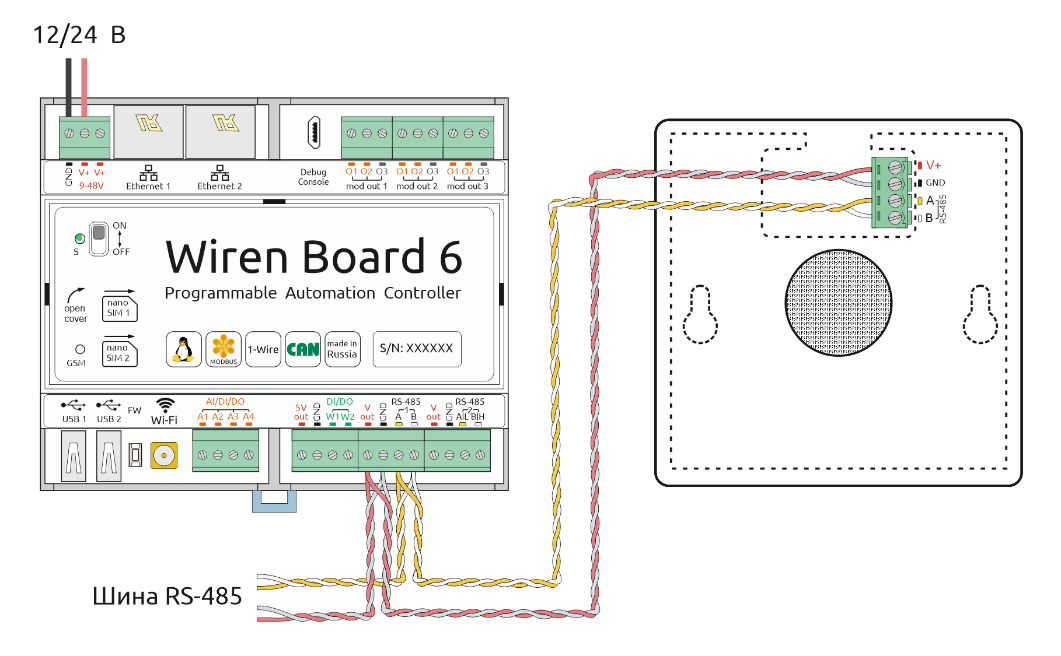
\includegraphics[width=0.5\linewidth]{images/device-4}
	\caption{Датчик движения}
	\label{fig:device-4}
\end{figure}

% TODO: \usepackage{graphicx} required
\begin{figure}[htpb]
	\centering
	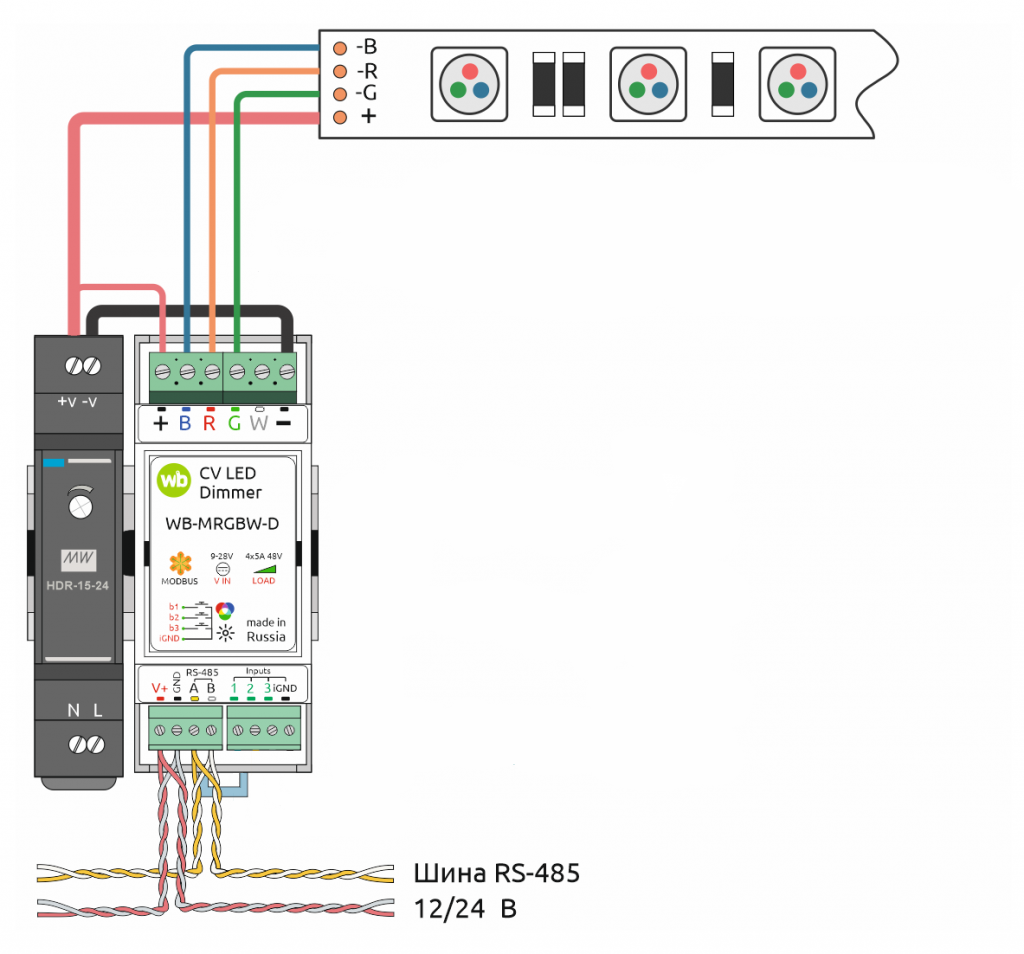
\includegraphics[width=0.5\linewidth]{images/device-5}
	\caption{Диммер светодиодных лент }
	\label{fig:device-5}
\end{figure}


\subsection{Технологии передачи данных}

В качестве технологий передачи данных от физического устройства в Интернет мы выбрали WiFi. Роутер WiFi есть у большинства пользователей Умного дома, что позволит сэкономить на необходимом оборудовании для установки. Также данный выбор обоснован низкими требованиями проекта. 


\section{Практическая работа №6.\\ Основы работы с протоколом MQTT. Брокераж сообщений }

\subsection{SHH-подключение}
Подключимся к консоли WirenBoard по протоколу SSH. Используем утилиту ssh. Работы будем проводить в оболочке PowerShell.
% TODO: \usepackage{graphicx} required
\begin{figure}[h!]
	\centering
	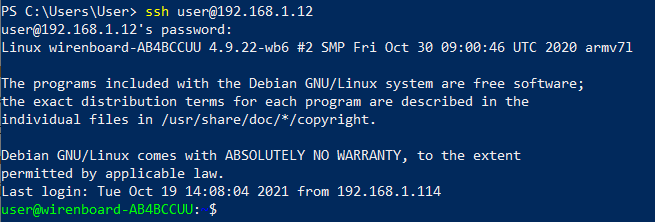
\includegraphics[width=0.9\linewidth]{images/ssh-powershell}
	\caption{Подключение к консоли WirenBoard по SSH}
	\label{fig:ssh-powershell}
\end{figure}
%
\subsection{Подписка на топик}

При помощи улиты mosquitto\_sub подпишемся на сообщения датчика влажности устройства WB-MS v.2 (12).
\newpage
% TODO: \usepackage{graphicx} required
\begin{figure}[htpb]
	\centering
	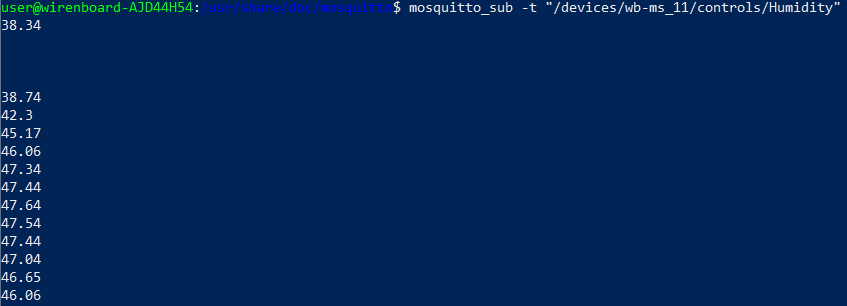
\includegraphics[width=0.9\linewidth]{images/ssh-powershell2}
	\caption{Подписка на сообщения датчика влажности}
	\label{fig:ssh-powershell2}
\end{figure}
При помощи улиты mosquitto\_sub подпишемся на сообщения кнопки 29.
% TODO: \usepackage{graphicx} required
\begin{figure}[htpb]
	\centering
	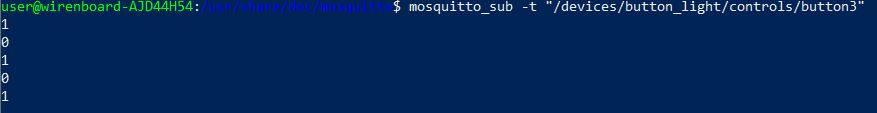
\includegraphics[width=0.9\linewidth]{images/ssh-powershell2.1}
	\caption{Подписка на сообщения кнопки 29}
	\label{fig:ssh-powershell2.1}
\end{figure}

\subsection{Управление устройствами}

Включим индикатор 26 посредством отправки сообщения в
соответствующий топик.
% TODO: \usepackage{graphicx} required
\begin{figure}[htpb]
	\centering
	
\includegraphics[width=1\linewidth]{images/ssh-powershell3.1}
	\caption{Включение индикатора 26}
	\label{fig:ssh-powershell3.1}
\end{figure}

\newpage
Изменим уровень громкости звукового сигнала посредством отправки сообщения в
соответствующий топик.

% TODO: \usepackage{graphicx} required
\begin{figure}[htbp]
	\centering
	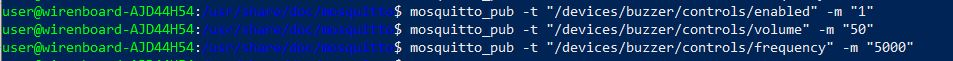
\includegraphics[width=0.9\linewidth]{images/ssh-powershell3.2}
	\caption{Изменение уровня громкости}
	\label{fig:ssh-powershell3.2}
\end{figure}
Проверим корректность изменений с помощью web-клиента.
% TODO: \usepackage{graphicx} required
\begin{figure}[htbp]
	\centering
	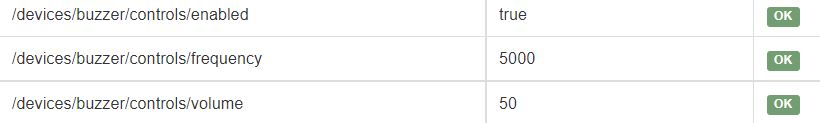
\includegraphics[width=0.8\linewidth]{images/ssh-powershell3.3}
	\caption{Сведения в web-клиенте}
	\label{fig:ssh-powershell3}
\end{figure}	

\subsection{Сообщения MQTT с внешнего устройства}

Настроим MQTT-мост (т.е. пересылку всех сообщений MQTT на любой облачный MQTT
брокер и обратно) (см. рис. \ref{fig:ssh-config}).
% TODO: \usepackage{graphicx} required
\begin{figure}[htbp]
	\centering
	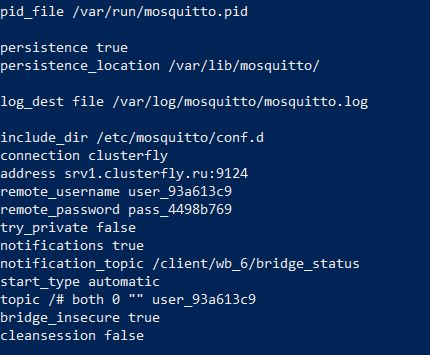
\includegraphics[width=0.6\linewidth]{images/ssh-powershell4}
	\caption{Настройка MQTT-моста}
	\label{fig:ssh-config}
\end{figure}

Наблюдаем изменение цвета RGB ленты в составе демонстрационного стенда \textbf{Wb-demo-kit v.2} (см. рис. \ref{fig:ssh-stend}). Данные изменения можно также увидеть в web-клиенте (см. рис. \ref{fig:ssh-web-client}).

% TODO: \usepackage{graphicx} required
\begin{figure}[htbp]
	\centering
	
\includegraphics[width=0.7\linewidth]{images/ssh-powershell4.2}
	\caption{Статус RGB контроллера в web-клиенте}
	\label{fig:ssh-web-client}
\end{figure}


% TODO: \usepackage{graphicx} required
\begin{figure}[htbp]
	\centering
	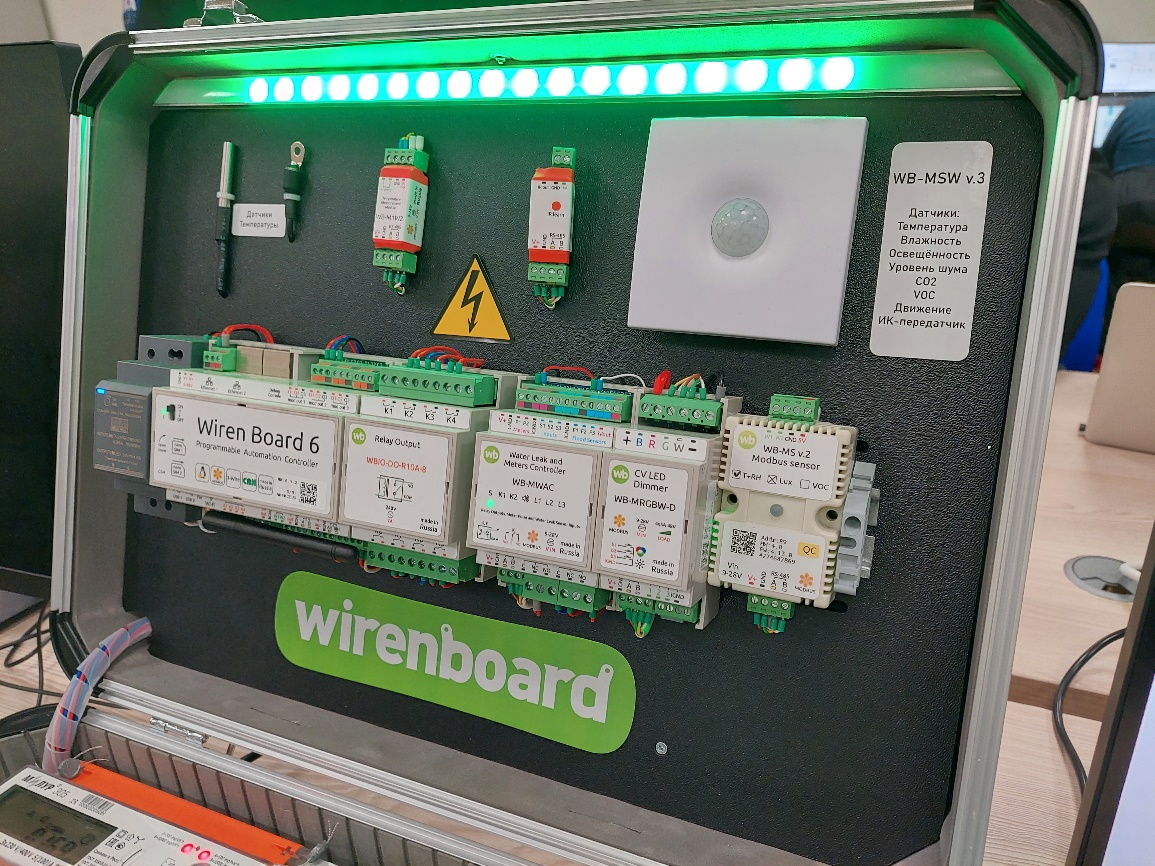
\includegraphics[width=0.6\linewidth]{images/ssh-powershell4.1}
	\caption{Изменения на стенде}
	\label{fig:ssh-stend}
\end{figure}
\newpage
\section{Дополнительные задания к работе №6}
\subsection{Выбор облачной платформы}
В качестве брокера сообщений и облачной платформы для них были выбраны Mosquitto и Clusterfly соответственно. Такой выбор исходит из нескольких причин:
\begin{itemize}
	\item Данные технологии распространяются свободно и отлично подходят для учебного проекта;
	
	\item В ходе выполнения предыдущих практических работ нами уже был получен опыт использования данных технологий, что облегчит их дальнейшее использование и увеличит скорость разработки проекта.
\end{itemize}


\subsection{Взаимодействие компонентов проекта}
Ниже приведена диаграмма последовательности взаимодействия сервисов проекта в методологии UML.
% TODO: \usepackage{graphicx} required
\begin{figure}[htpb]
	\centering
	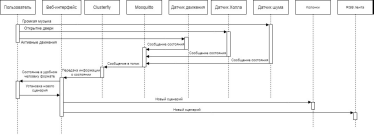
\includegraphics[width=0.9\linewidth]{images/sql}
	\caption{Диаграмма последовательности взаимодействия}
	\label{fig:sql}
\end{figure}








\newpage
\end{document}


